% !TEX root = ../../main.tex

\subsubsection{UiO-66(Zr)}

A visual inspection of the enthalpy curves on as-synthesised UiO-66(Zr)
show it to be relatively homogenous, with flat
profiles being common. This is typical of this MOF, which has
a pore environment without high energy adsorption sites
~\cite{wiersumEvaluationUiO66GasBased2011}.
Both \ce{CO2} and \ce{CO} show a higher enthalpy of adsorption
at low loadings, as seen in \autoref{shaping:fig:uio66isotherms},
which is likely due to their quadrupole and dipole interaction,
respectively.

\begin{figure}[p!]
	\centering
	\begin{subfigure}{\linewidth}
		\parbox[c]{0.1\linewidth}{\caption{}%
			\label{shaping:fig:analysisuio66henry}}%
		\parbox[b]{0.8\linewidth}{%
			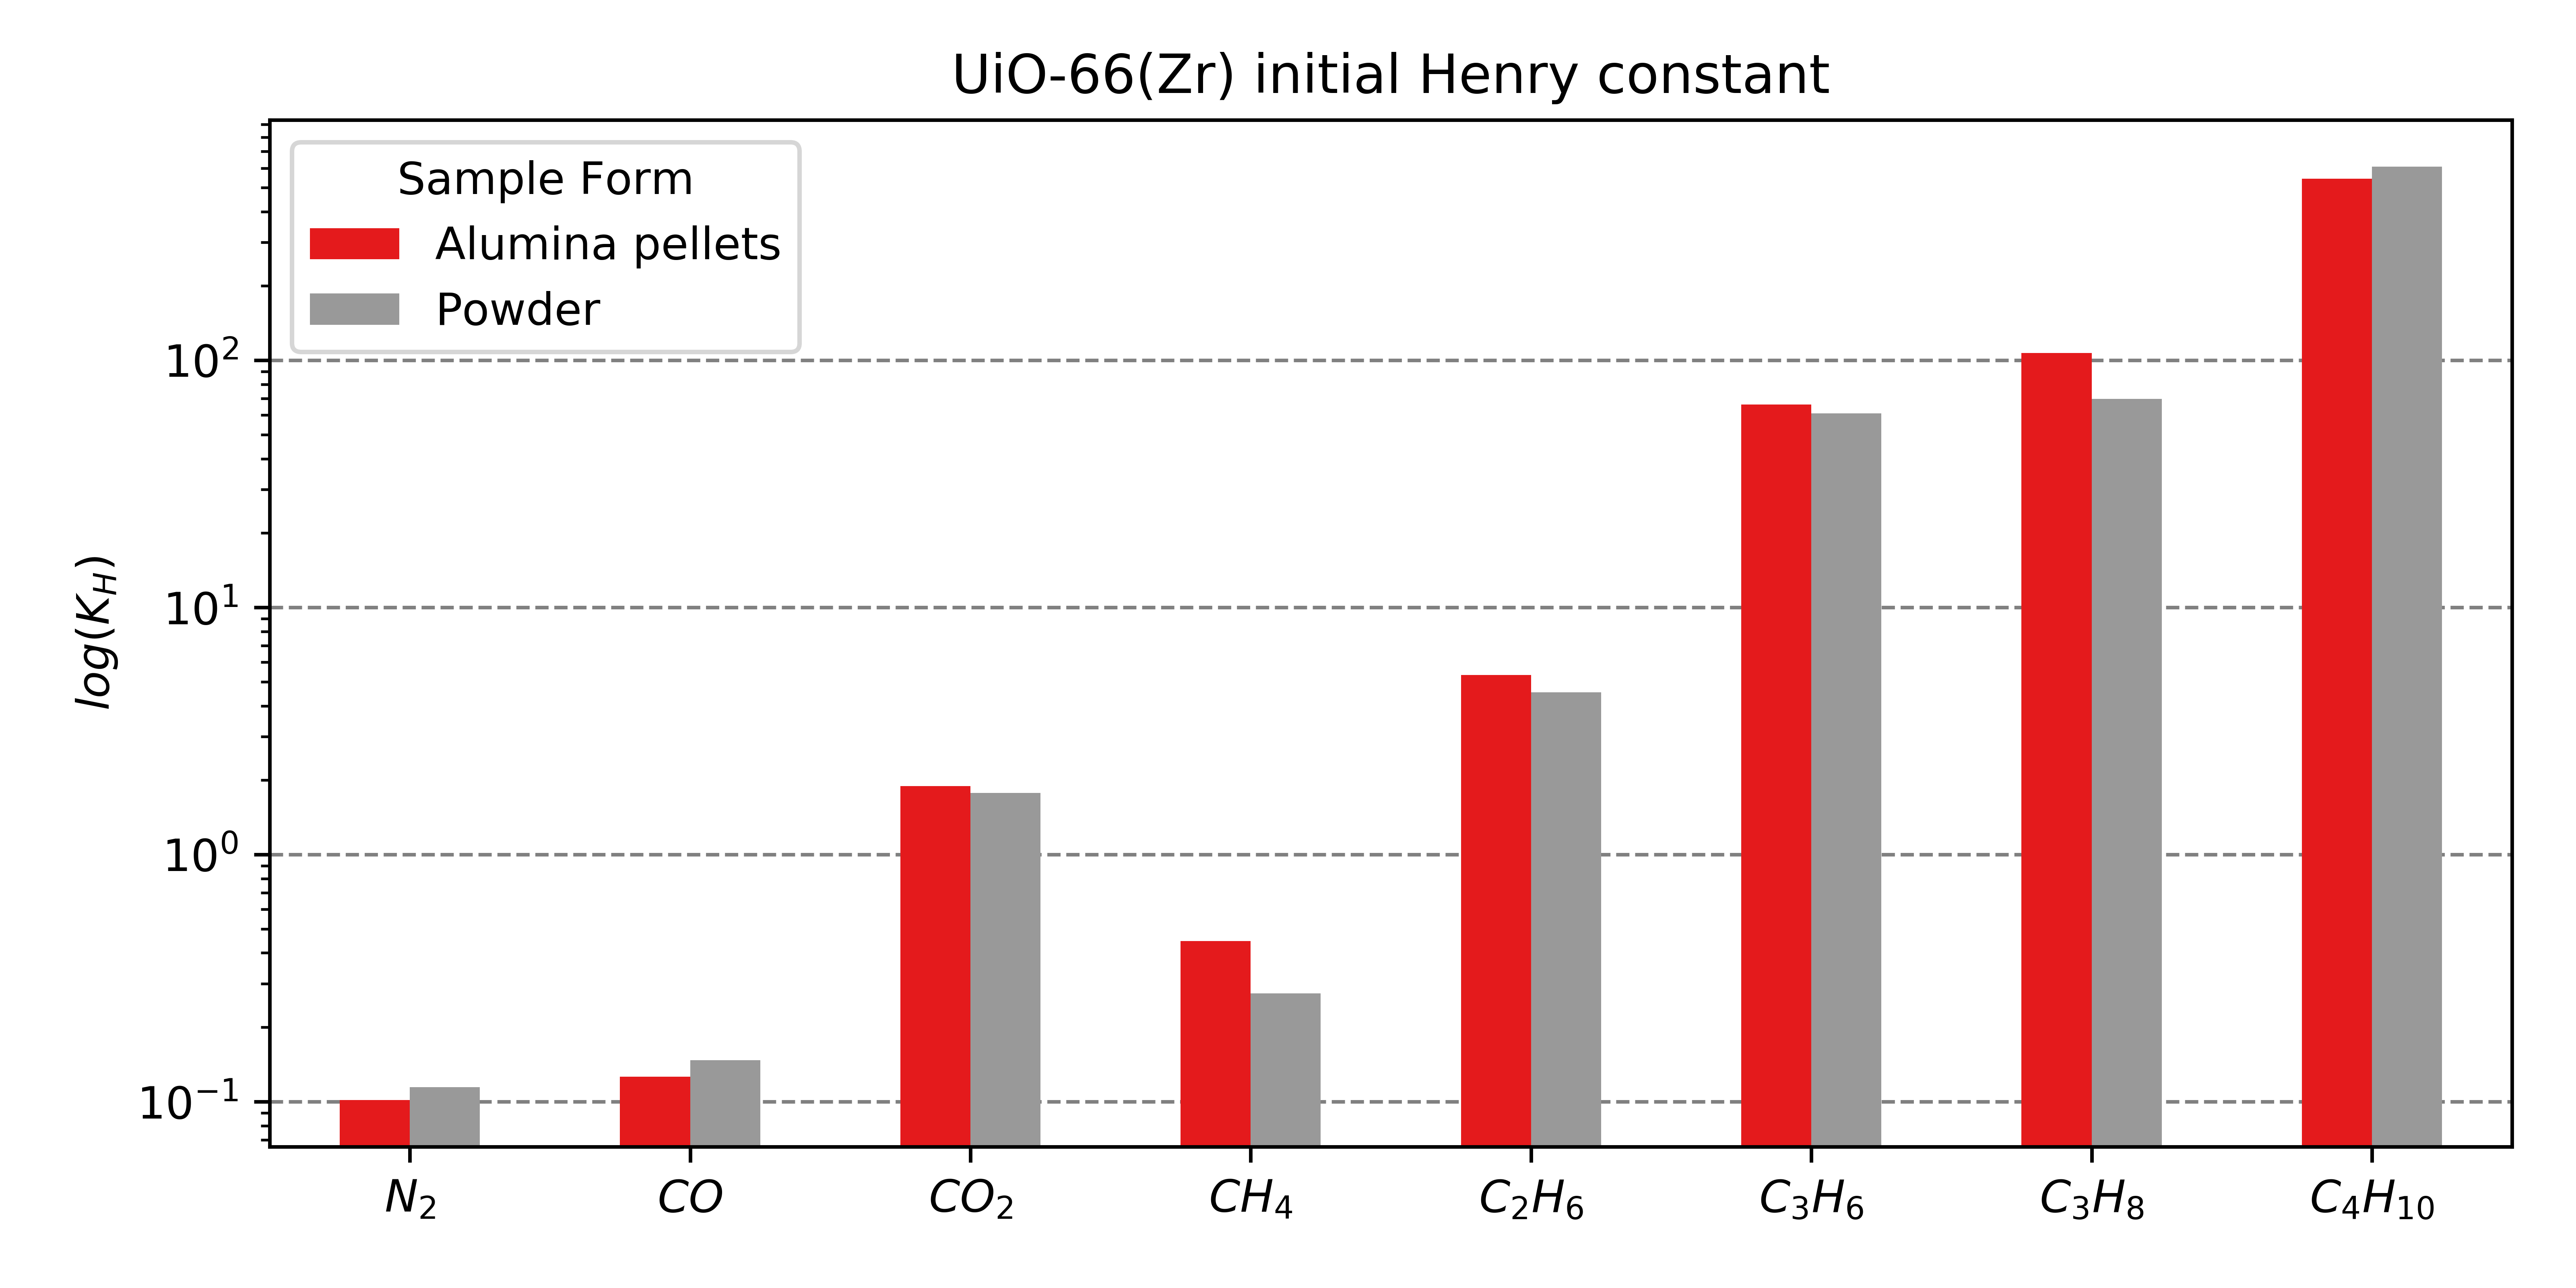
\includegraphics[width=\linewidth]{UiO-66(Zr)-henry-distribution}%
		}%
	\end{subfigure}%

	\begin{subfigure}{\linewidth}
		\parbox[c]{0.1\linewidth}{\caption{}%
			\label{shaping:fig:analysisuio66enth}}%
		\parbox[b]{0.8\linewidth}{%
			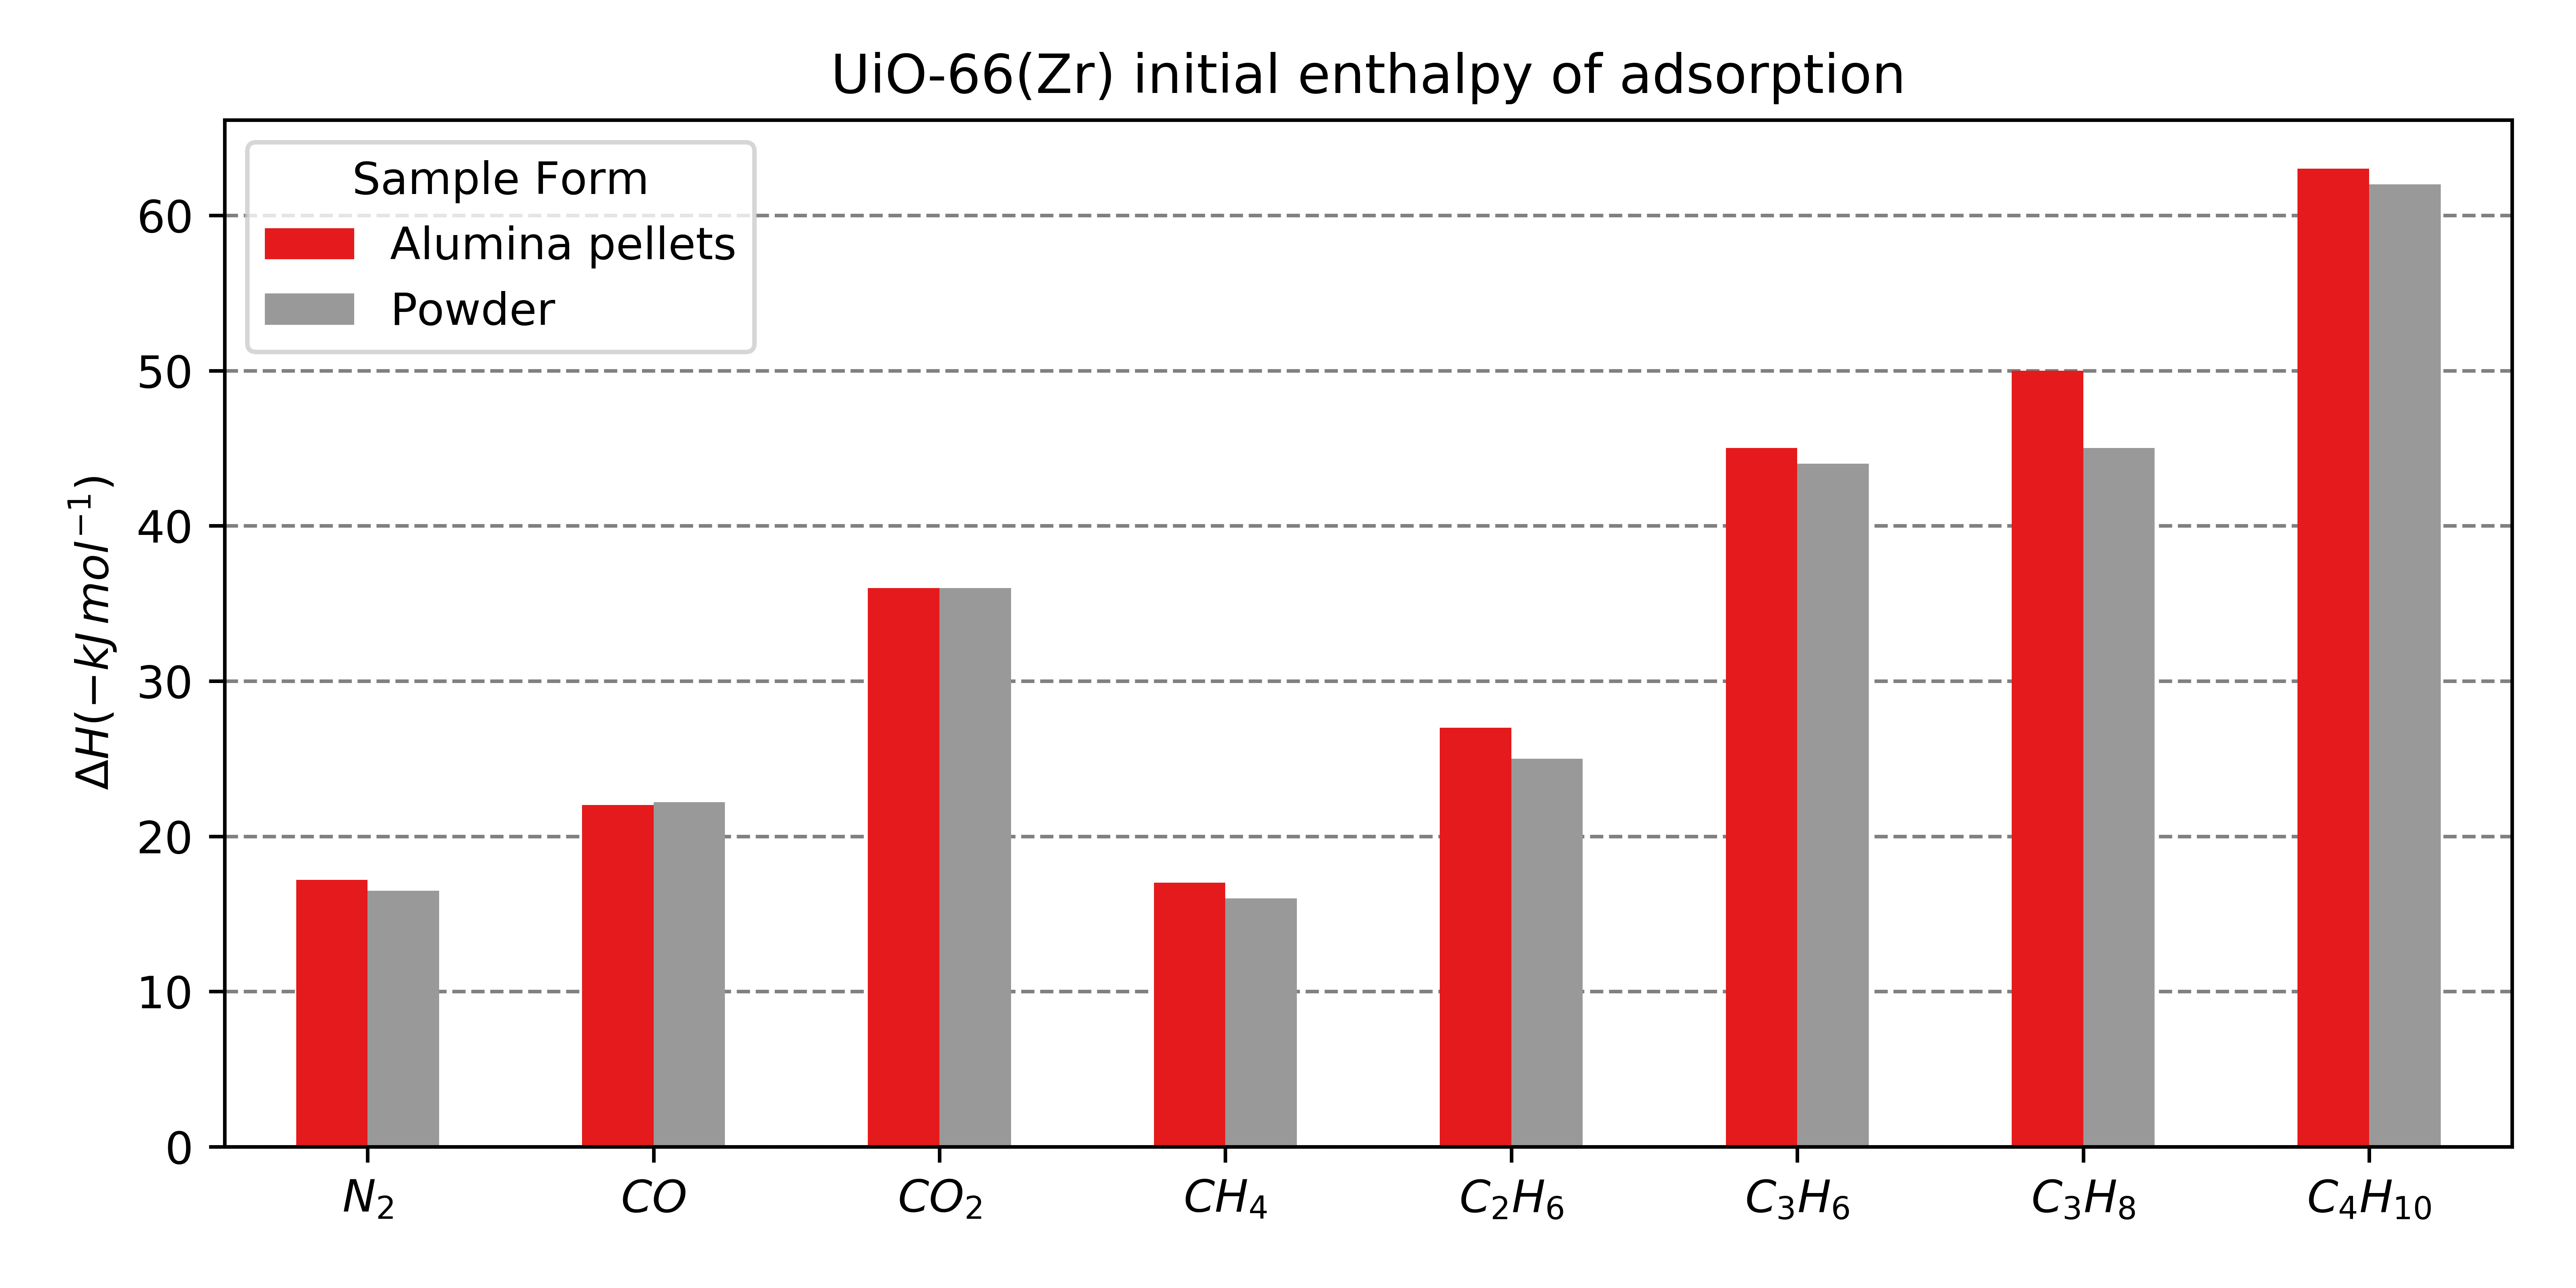
\includegraphics[width=\linewidth]{UiO-66(Zr)-enthalpy-distribution}%
		}%
	\end{subfigure}%

	\begin{subfigure}{\linewidth}
		\parbox[c]{0.1\linewidth}{\caption{}%
			\label{shaping:fig:analysisuio66basis}}%
		\parbox[b]{0.8\linewidth}{%
			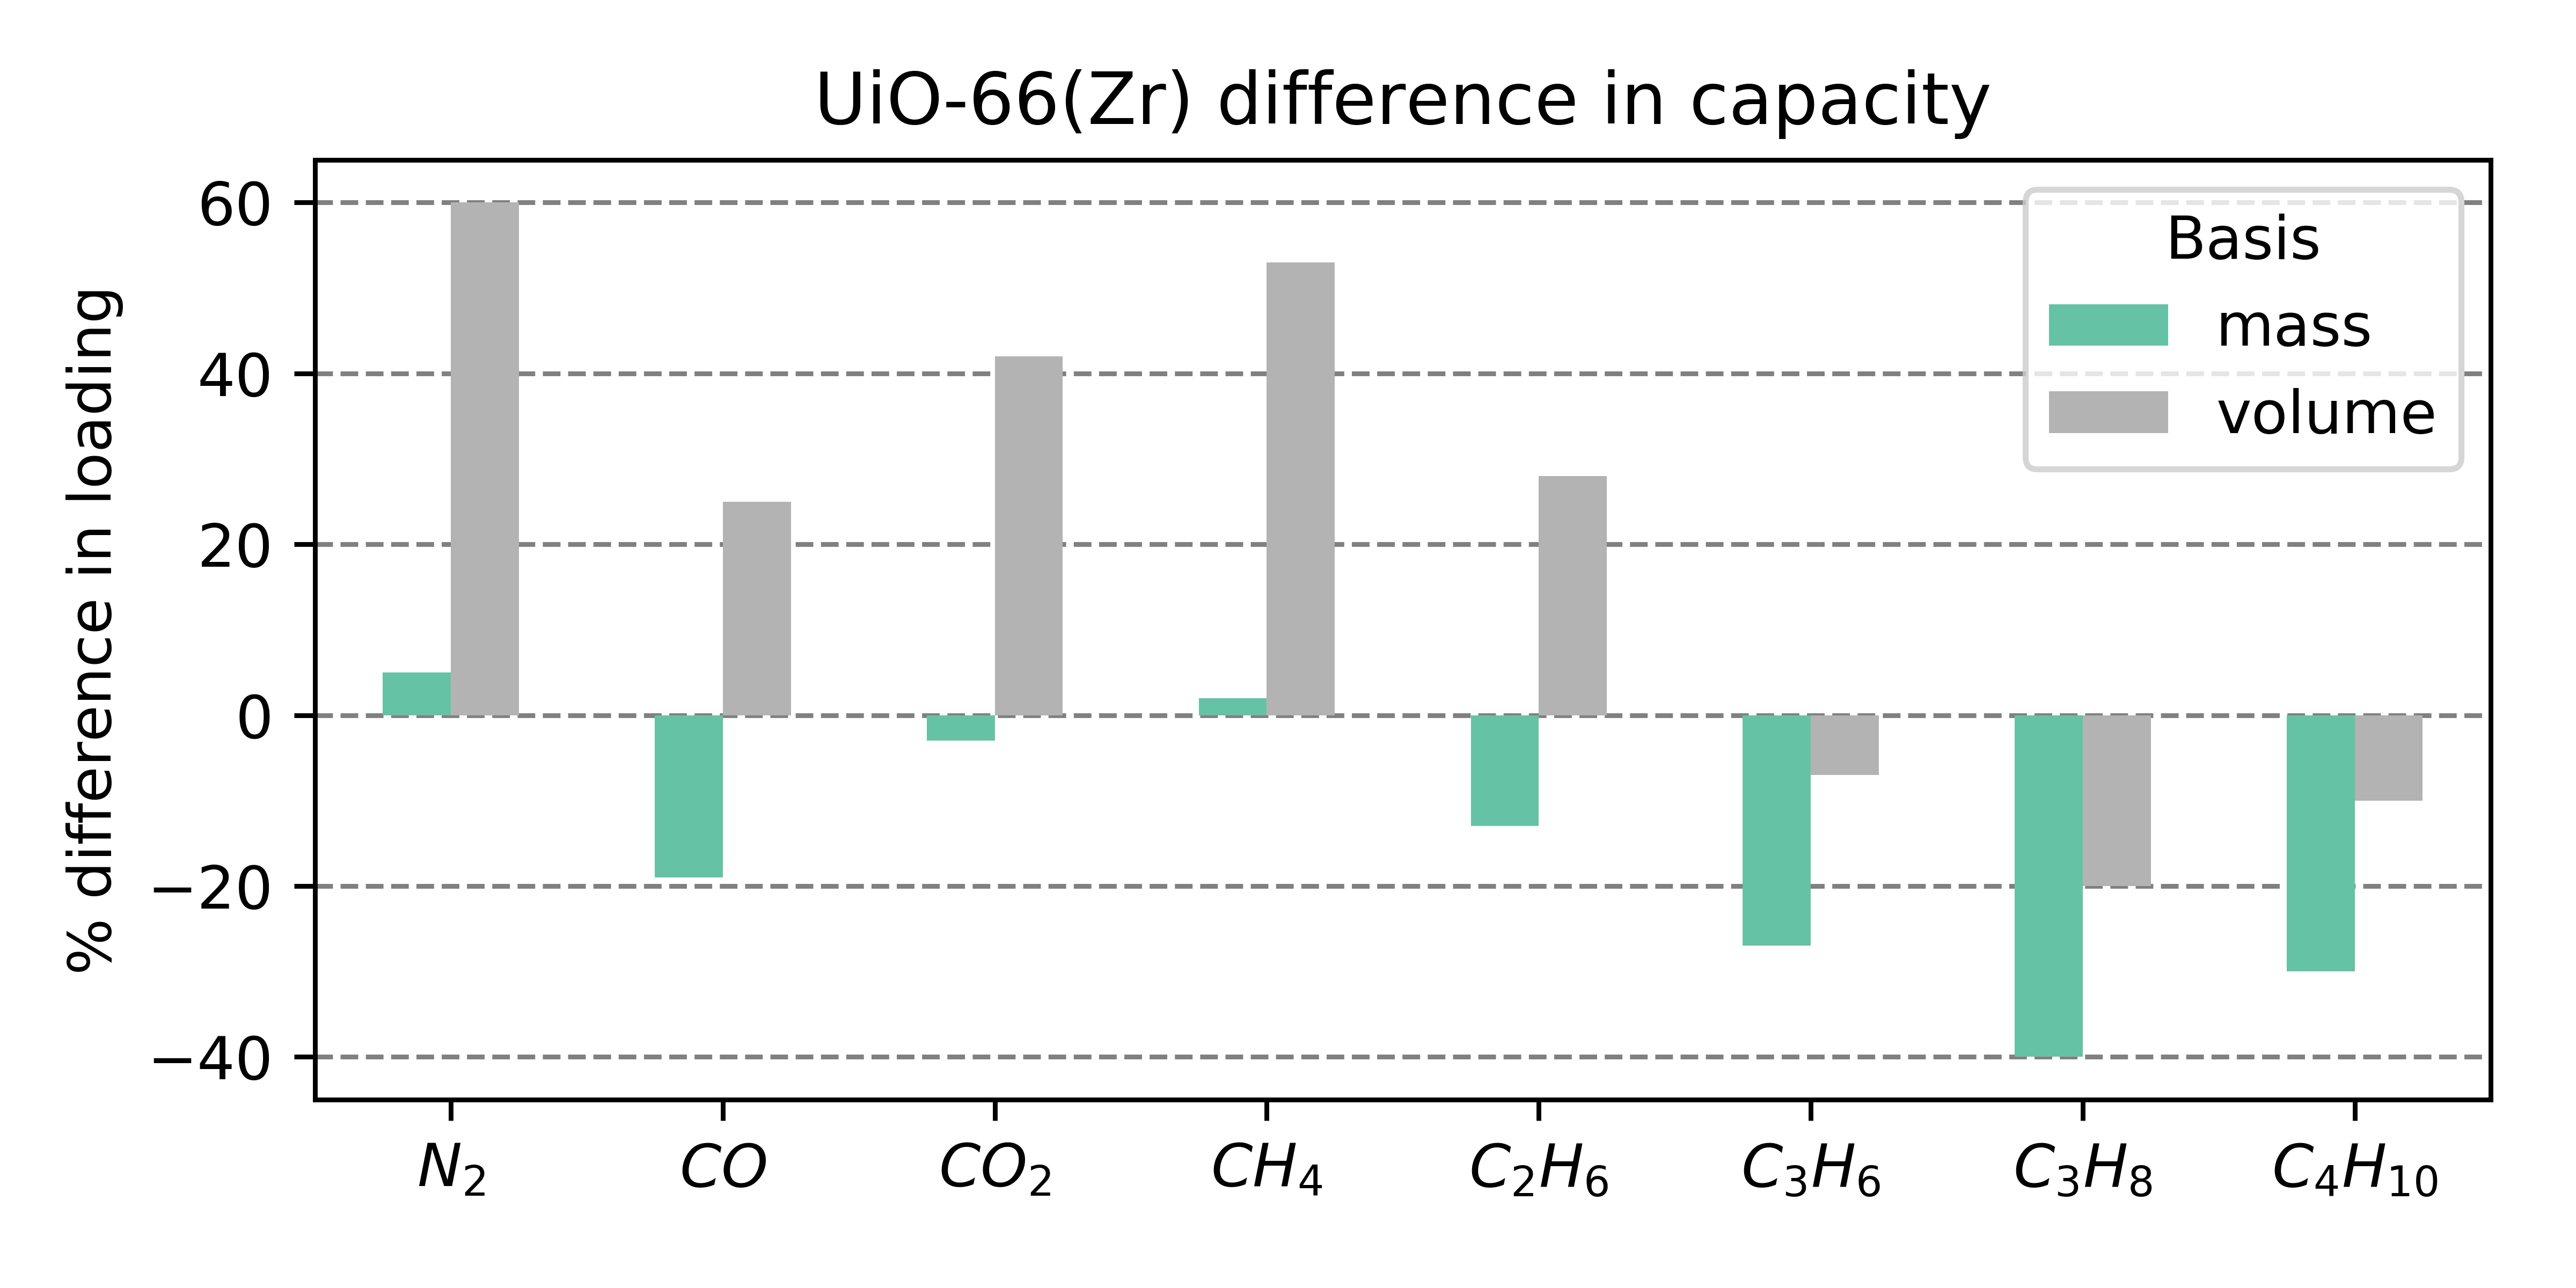
\includegraphics[width=\linewidth]{UiO-66(Zr)-mass-volume}%
		}%
	\end{subfigure}%

	\caption{KPIs extracted from the UiO-66(Zr) adsorption dataset with
		(a) logarithmic initial Henry constant (b) initial enthalpy of
        adsorption and (c) change in adsorption maximum capacity from 
        the powder to the alumina shaped version on a mass and volume 
        basis in red and grey respectively}%
	\label{shaping:fig:analysisuio66}
\end{figure}

\begin{figure}[htb]
	\centering
	\begin{subfigure}{0.45\textwidth}
		\includegraphics[width=\linewidth]{calo/UiO-66(Zr)/co2-mass-basis-iso}
		\caption{\ce{CO2} adsorption isotherms}%
		\label{shaping:fig:uio66co2ads}
	\end{subfigure}%
	\begin{subfigure}{0.45\textwidth}
		\includegraphics[width=\linewidth]{calo/UiO-66(Zr)/co-mass-basis-iso}
		\caption{\ce{CO} adsorption isotherms}%
		\label{shaping:fig:uio66coads}
	\end{subfigure}%
	\caption{Selected isotherms from the UiO-66(Zr) dataset}%
	\label{shaping:fig:uio66isotherms}
\end{figure}

The KPI graphs in \autoref{shaping:fig:analysisuio66} show very
similar values for both initial Henry's constant and initial
enthalpy of adsorption. It is therefore apparent that the shaping process
did not change the interaction of the adsorbate with the MOF surface.

The maximum capacity graphs show a more interesting trend.
When using small adsorbates such as \ce{N2}, \ce{CO2} and \ce{CH4},
the shaped samples have a similar performance on a mass basis and,
due to the densification process, better capacities on a volume
basis. Starting with ethane, the maximum capacity difference starts
to increase, with lower performance as molecule size increases.
On hydrocarbons with a carbon number of 3 and 4, both mass basis and
volume basis capacity are decreased compared to the original powder.
This size exclusion effect could be explained by the coating of
crystal surfaces with the alumina binder.

It could also be argued that instead of size exclusion, the effect is due to
an overall decrease in pore volume, and that the isotherms of the
low molecular weight gasses will diverge at higher pressures
as the pores are filled. A counterargument for this hypothesis is that
in the case of \ce{CO2}, the plateau is reached with no differences
between the powder and the pellet as seen
in \autoref{shaping:fig:uio66co2ads}.

Carbon monoxide is an apparent outlier to this trend, with a
decreased maximum capacity and a small molecular size.
However, when observing the isotherms directly
(\autoref{shaping:fig:uio66coads}) it is obvious that the effect is
likely to be due to experimental errors, considering
the low amount adsorbed and the good overlap in the enthalpy
curves.

Overall, the shaping performance of UiO-66(Zr) is
reasonable, as long as only small adsorbates are used.
